% Numerical content is generated from the checksum-verified 60 Hz v5 formal result.
% Existing references.bib entries are used without modification.
\chapter{Experimental Evaluation}
\label{chap:experimental_evaluation}
\input{experiment_results/reanalysis_rescue_60_v5/chapter6_numbers.tex}

\section{Experimental Questions and Protocol}

This chapter evaluates Humanoid Matcher as a retrieval-based music-to-motion
system with continuous kinematic playback. It separates the quality of the
selected motion from the quality and timeliness of its execution. A fast
catalogue search does not establish a fast musical response, and a bounded
intermediate joint command does not establish that the final displayed pose
satisfies the same bounds.

Five research questions organise the evaluation:
\begin{enumerate}
    \item RQ1: does the catalogue support meaningful retrieval for unseen music,
          and can unsuitable inputs be rejected?
    \item RQ2: does beat-synchronised timing improve rhythm alignment, and does
          the selection policy maintain diversity without losing relevance?
    \item RQ3: are motion transitions and final outputs continuous and within
          the specified kinematic and clearance constraints?
    \item RQ4: which computational stages dominate latency, and does the
          complete system meet its real-time operating targets?
    \item RQ5: which component contributions are supported by controlled
          ablations and long-duration operation?
\end{enumerate}



\section{Datasets, Splits and Reproducibility}

The local catalogue contains 60 music identities, 348 descriptor segments and
411 selectable motions spanning ten AIST++ genres. These are the assets
available to this implementation, not the complete AIST++ dataset
\cite{li2021ai}. Strict leave-one-music-out evaluation removes every descriptor,
track record and motion associated with the query music identity before ranking.
The 60 music identities define the
independent units of this retrieval evaluation.

The literature-oriented subset freezes four music identities per genre. Each
music identity is paired with its lexicographically first preflight-passed
ground-truth motion. Five seeds yield 200 outputs. The evaluation excludes six
seconds of warm-up and reconstructs the following 20 seconds at 60 frames per
second. The full-system suite evaluates all 60 catalogue music identities and
ten CC0 recordings at five seeds. Unlike strict leave-one-music-out retrieval,
these runtime suites exercise the deployed catalogue without imposing an
unseen-music exclusion on every run. They must not be interpreted as additional
held-out retrieval tests.

The causal short suite compares the full system with authored timing on the
same 13 inputs: the stitched AIST++ recording, ten CC0 recordings, a tempo jump,
and a silence/recovery stream. Each condition has 65 runs of 40 seconds, including
six seconds of warm-up. Five full-system long runs use 606-second inputs, giving
approximately 600 seconds of post-warm-up observation per seed. Short source
recordings are deterministically repeated when necessary. In particular, the
stitched source has a 39-second cycle because of its crossfades. Its repetition
boundary is itself a musical change, not a seamless continuation.

The rejection evaluation includes the ten CC0 inputs and 20 synthetic negative
inputs, with 750 overlapping query windows in total. The negatives comprise
silence, pink noise, ambient drones and speech-like signals. They constitute a
synthetic stress test, not coverage of recorded human speech or environmental
sound. The window-level rejection scores below are descriptive. Adjacent windows
are not treated as 750 independent recordings.

The new causal formal experiments are serial, headless and configured for a
60 Hz control loop, a six-second matching window and a one-second matching
interval. Seeds are fixed to 0--4. A separate frozen 21-run pilot evaluates the
original 120 Hz target: only six runs pass all gates, with worst control-work
p99 of 15.572 ms and worst deadline-miss ratio of 0.18544. It is retained as a
capacity test and is not pooled with the 60 Hz formal cohort. The recorded
platform has 20 logical CPU cores and an RTX 3080,
but ONNX inference uses \texttt{CPUExecutionProvider} exclusively. Python 3.11.14,
NumPy 1.26.4, librosa 0.10.2.post1, ONNX Runtime 1.28.0, SciPy 1.11.4 and MuJoCo
3.10.0 are recorded in the manifest. The GPU model is not evidence of GPU
inference.

Every supplemental run preserves its command, source identity, seed, trace,
timing report, final-pose archive and log. The audit checks the registered run
matrix, artifact hashes, strictly increasing output clocks and consistent robot
identity. All 538 frozen input-file hashes matched during the post-run audit.
The supplemental index contained no failed attempts. Original and supplemental
provenance are retained separately even though both record the same Git commit:
the source-file hashes also capture uncommitted implementation changes.

\section{Evaluation Metrics}

\subsection{Retrieval, rejection and statistical units}

Genre Recall@$K$, macro-$F_1$, mean reciprocal rank (MRR) and NDCG@5 measure
catalogue matching. Source motion recall is retained only as an internal
same-catalogue sanity check. It cannot establish generalisation because the
target and candidates share catalogue provenance. CC0 genre labels are sets of
acceptable catalogue genres, rather than an exhaustive taxonomy of the recordings.

For runtime quality metrics, frames are first reduced to a run summary. Seeds
are then averaged within each source recording. Confidence intervals use 2,000
bootstrap resamples of source means. Ablations use two-sided paired sign-flip
permutation tests after averaging matched seeds within each source. Holm
correction covers the reported condition-by-metric tests within each suite.
The direction of a mean difference alone is not evidence of a component benefit.
For the long-run suite, five seeds of one repeated source quantify repeatability. A one-source bootstrap interval is
degenerate and must not be read as strong generalisation evidence.

\subsection{Rhythm and motion diversity}

Following the beat-alignment evaluation family used in dance generation
\cite{li2021ai,siyao2022bailando}, this chapter defines the music-to-dance score as
\begin{equation}
 A_{m\rightarrow d} = \frac{1}{|B_m|}\sum_{t\in B_m}
 \exp\!\left(-\frac{\min_{u\in B_d}(u-t)^2}{2\sigma^2}\right),
 \qquad \sigma=\frac{3}{60}\;\mathrm{s}.
\end{equation}
The reverse score is calculated by exchanging the beat sets. Their harmonic
mean is the main BAS summary. Robot output is resampled to 60 FPS. Motion beats
are local minima of mean body-speed magnitude, with a minimum separation of
0.20 seconds. The stationary MuJoCo world body is excluded and the pelvis is
used as the positional reference. 

For causal runs, $B_m$ contains the actual delivery times of all online detected
beats, not retrospectively estimated beat times and not only the subset accepted
by the phase controller. Consequently the score assesses alignment to delivered
control information, not accuracy against an annotated musical beat ground truth.
When no music beats are available, BAS is undefined and excluded from numerical
averages with its missingness retained. Preanalysed replay uses its original beat
records and is reported separately.

Kinetic and geometric FID/Div are calculated in reconstructed AIST++/SMPL space
using the pinned feature implementation. Each seed is evaluated against the same
40 ground-truth items. Div uses all 780 unordered pairs. Both raw feature scale
and standardisation using ground-truth means and standard deviations are made
explicit. Robot-domain diversity additionally reports unique selected motions,
catalogue-cluster coverage and normalised selection entropy. This entropy is
computed over \emph{selection episodes}, after collapsing consecutive identical
motion IDs. It is not a dwell-time-weighted entropy. Catalogue clusters are
engineered motion descriptors, not human judgements of visual style.

\subsection{Continuity, contact and constraints}

Final joint positions are read from MuJoCo qpos after limiting, collision
projection and joint-range clipping. Velocity uses successive actual wall-clock
differences. Acceleration and jerk use the corresponding midpoint clocks.
The old cohort lacks such frame clocks, so its nominal-rate derivatives are
diagnostics only. They are not reconstructed physical-time measurements.

The safety audit distinguishes candidate clearance detections, corrective
projections and violations remaining in the final pose. The configured clearance
target is 6 mm, comprising the existing 5 mm minimum plus a 1 mm buffer. A residual
clearance violation therefore does not, by itself, prove geometric penetration.
Conversely, a correction count is not a residual violation count. Both are useful
but answer different questions.

Physical Foot Contact (PFC) was introduced to assess dance plausibility
\cite{tseng2023edge}. The old COM/foot-speed formula is retained only as a legacy
proxy. The new G1 adaptation follows the official evaluator's algebra on a
30 FPS grid. The magnitude of root acceleration, after clamping its downward
component, is normalised by its sequence maximum and multiplied by the horizontal
displacements of the two feet. The result is averaged and scaled by $10^4$.
Unlike the SMPL implementation's ankle/toe minima, G1 uses one recorded body
anchor per foot. Zero root acceleration is assigned zero score instead of an
undefined division. These explicit differences preclude direct numerical
comparison with published SMPL PFC results. Foot skating and support-height
diagnostics are also retained in the machine-readable results.

\section{Retrieval and Rejection Results}

\begin{table}[tb]
\centering\small
\input{experiment_results/reanalysis_rescue_60_v5/chapter6_tables/retrieval.tex}
\caption{Strict leave-one-music-out genre retrieval (60 music identities) and
descriptive window-level rejection (750 windows from 30 recordings)}
\label{tab:ch6_retrieval}
\end{table}

Recall@1 is \ChSixRecallOne{}, whereas Recall@5 reaches \ChSixRecallFive{}
(Table~\ref{tab:ch6_retrieval}). Relevant genre information is therefore more
reliably retained in a shortlist than selected as the single best answer. The
results support a useful retrieval signal, but not consistently correct genre
identification for previously unseen music.

\begin{table}[tb]
\centering\small
\input{experiment_results/reanalysis_rescue_60_v5/chapter6_tables/genre.tex}
\caption{Per-genre leave-one-music-out results. Each genre has six music
identities}
\label{tab:ch6_genres}
\end{table}

The per-genre results in Table~\ref{tab:ch6_genres} prevent the overall average
from obscuring genre-dependent failure. The rejection AUROC is
\ChSixRejectAuroc{}. The operating-point precision and recall must be considered
alongside that ranking score and the unequal number of positive and negative
windows. Precision alone does not establish robust rejection.

\begin{table}[tb]
\centering\scriptsize
\input{experiment_results/reanalysis_rescue_60_v5/chapter6_tables/cczero.tex}
\caption{Per-recording CC0 results from offline query evaluation. Genre hit rate
uses the registered acceptable-genre sets. Ambient audio has no positive genre
target. Overlapping windows within a recording are descriptive repeats.}
\label{tab:ch6_cczero}
\end{table}

Table~\ref{tab:ch6_cczero} reports each CC0 recording rather than treating ten
heterogeneous inputs as a large domain-generalisation benchmark. Together, the
retrieval and rejection results answer RQ1 partially: the catalogue provides
useful candidates, but neither top-one matching nor rejection is sufficiently
reliable to serve as an unqualified deployment guarantee.

\section{Rhythm, Diversity and Physical Plausibility}

\begin{table}[tb]
\centering\scriptsize
\input{experiment_results/reanalysis_rescue_60_v5/chapter6_tables/rhythm.tex}
\caption{Source-averaged rhythm and adapted physical-contact scores. $N$ is the
number of runs, not the bootstrap sample size. Replay and causal BAS use different
beat-information protocols. Their difference is not a controlled causal effect.
The long-run interval has only one source and is not a population-level CI.}
\label{tab:ch6_rhythm}
\end{table}

\begin{figure}[tb]
\centering
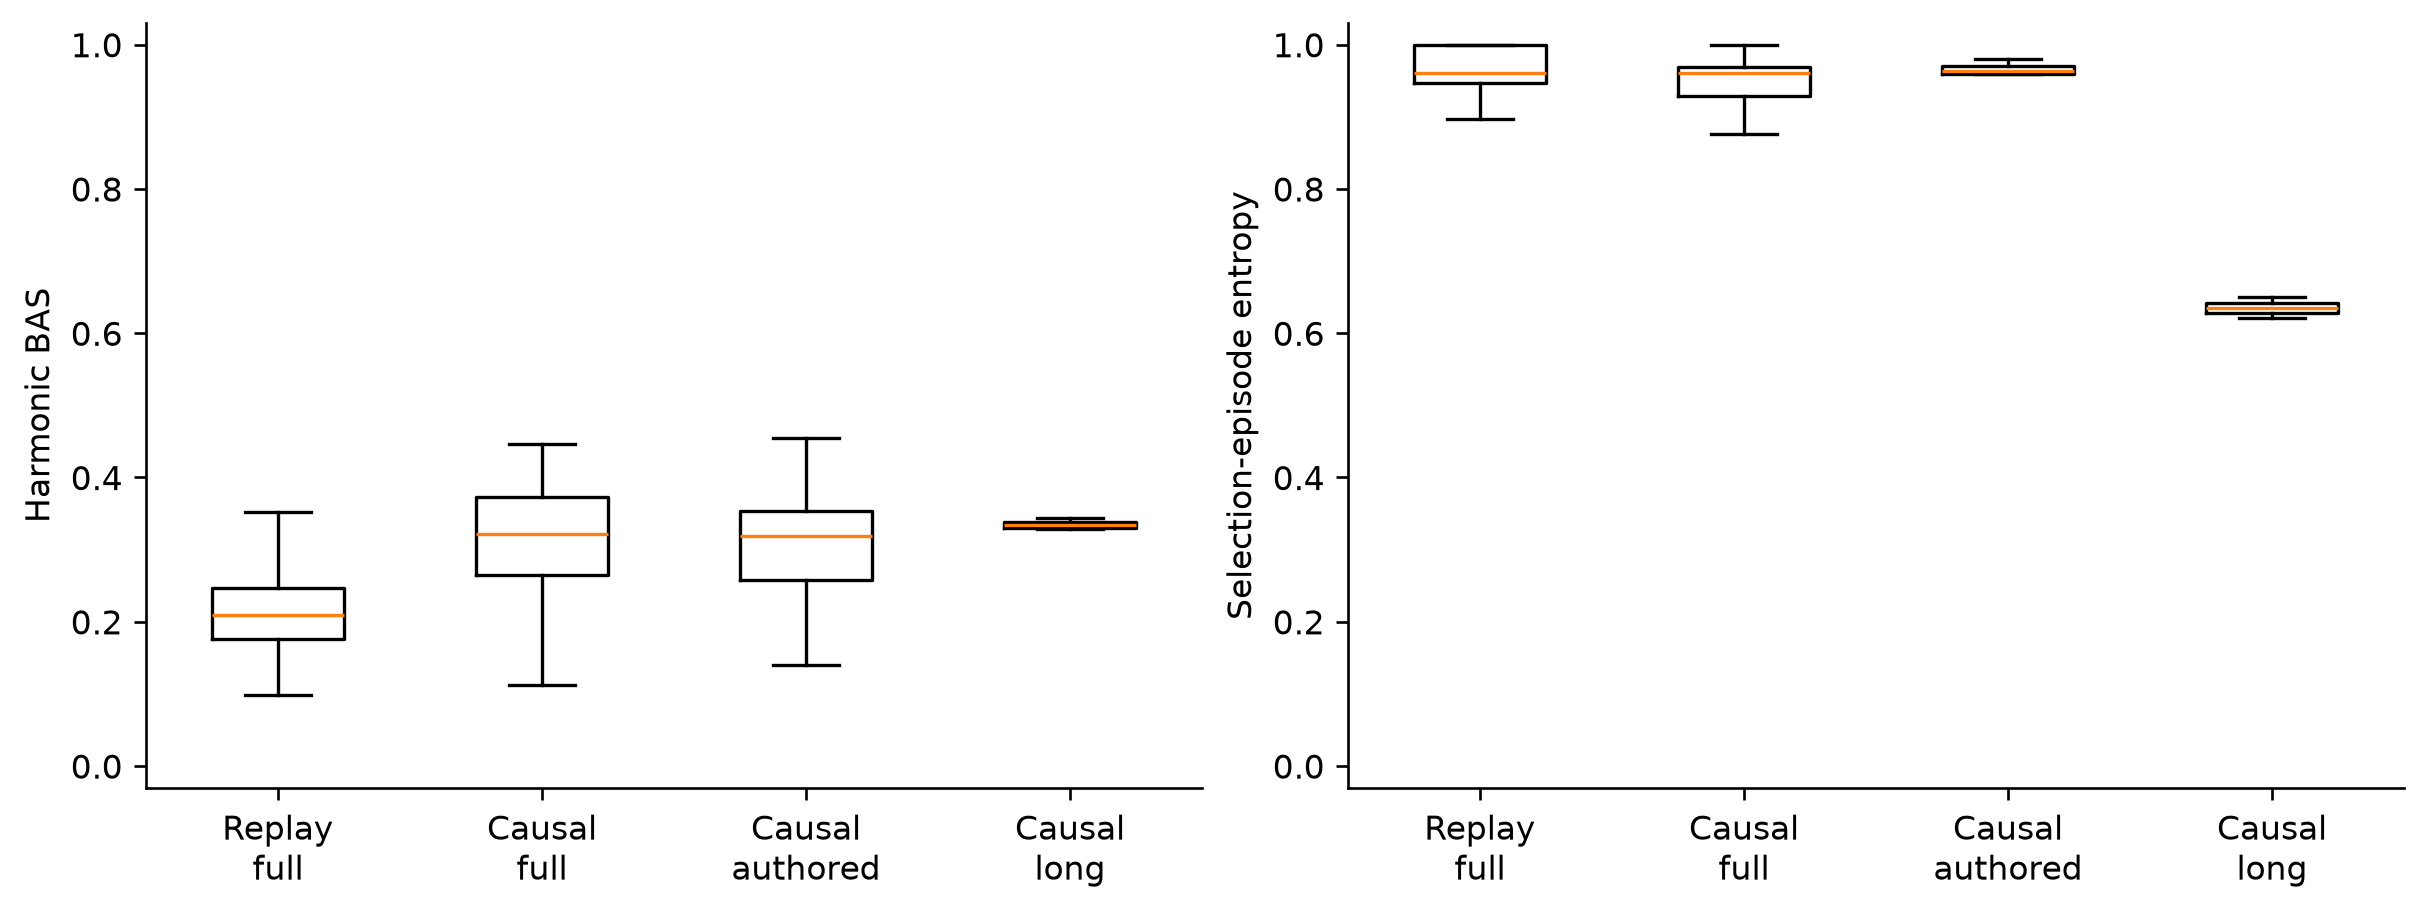
\includegraphics[width=\linewidth]{figures/chapter6_rhythm_diversity.png}
\caption{Distributions of run-level BAS and selection-episode entropy. }
\label{fig:ch6_rhythm}
\end{figure}

Table~\ref{tab:ch6_rhythm} and Figure~\ref{fig:ch6_rhythm} expose variability
that would be hidden by reporting a single BAS. The valid timing ablation is
full versus authored within the causal short suite: sources, seeds, input lengths
and measurement instruments are matched. Comparing the original replay cohort
with the causal cohort would simultaneously change beat information, output-clock
measurement and safety-audit overhead.

In the matched causal comparison, full-system harmonic BAS is
\ChSixFullBas{}, compared with \ChSixAuthoredBas{} for authored timing.
The full-minus-authored gain is \ChSixBasGain{} with a source-bootstrap 95\%
interval of [\ChSixBasGainLow{}, \ChSixBasGainHigh{}]. The interval includes
zero and the Holm-adjusted permutation $p$-value is \ChSixBasHolm{}. The formal
causal evidence therefore does not establish that beat-synchronised timing
improves BAS relative to authored timing under this delivered-beat metric.

\begin{table}[tb]
\centering\scriptsize
\input{experiment_results/reanalysis_rescue_60_v5/chapter6_tables/features.tex}
\medskip

\input{experiment_results/reanalysis_rescue_60_v5/chapter6_tables/groundtruth_div.tex}
\caption{Reconstructed SMPL feature metrics: mean and standard deviation over
five separate 40-output seed evaluations. Ground-truth Div is supplied as a
reference, not a value to exceed. Raw and standardised feature scales must not
be mixed in comparisons.}
\label{tab:ch6_features}
\end{table}

Table~\ref{tab:ch6_features} is deliberately a within-protocol characterisation,
not a leaderboard comparison. Trace phases and blend factors are interpolated
within unchanged motion/transition segments, while categorical switch boundaries
are handled separately. Reconstruction aligns root translation but cannot recover
every sub-trace boundary or the robot's final yaw, limiting and projection effects.
Short ground-truth motions are cycled, potentially introducing root seams. Finally,
the system retrieves real source motions, whereas an unconstrained generator must
produce its own trajectories. These differences can bias FID and Div, and diversity
is interpreted relative to the reference distribution.

The raw geometric Div is only \ChSixGeomDivRatio{} of the ground-truth value,
indicating a narrower reconstructed geometric feature distribution. More
importantly, some ground-truth geometric dimensions have zero variance. Dividing
output deviations by the implemented $10^{-8}$ standard-deviation floor produces
the extremely large standardised geometric values in Table~\ref{tab:ch6_features}.
Those entries diagnose ill-conditioned normalisation, not a meaningful ranking
of dance quality. They are not used as a primary success criterion. The large
raw kinetic scale and its seed variability must also be read alongside the
cyclic-source and reconstruction limitations, rather than compared directly with
published generation benchmarks.

\begin{figure}[tb]
\centering
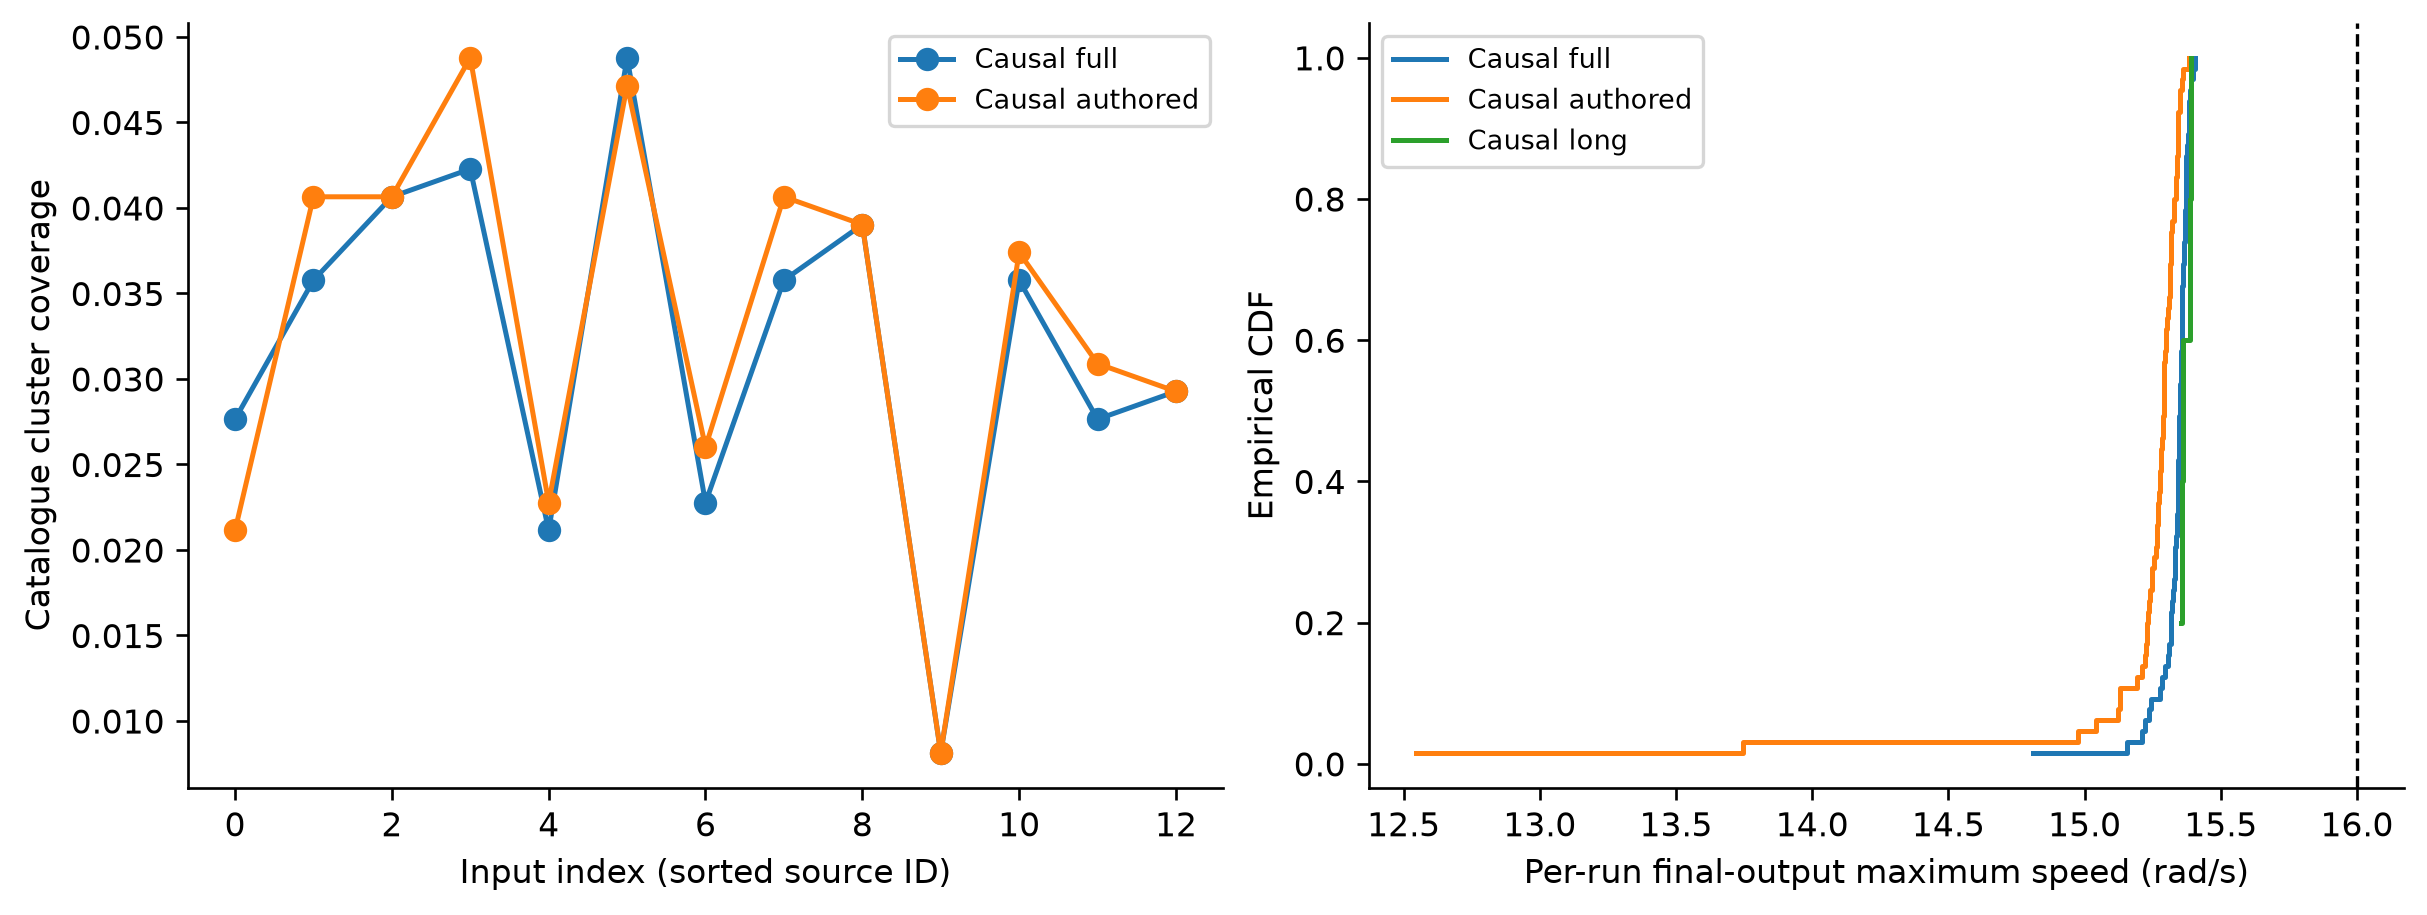
\includegraphics[width=\linewidth]{figures/chapter6_coverage_safety.png}
\caption{Left: mean catalogue-cluster coverage across five seeds per causal
short-suite input, ordered by source ID. Right: empirical distributions of
per-run maximum final-output speed. The dashed line is the 16 rad/s target.
Coverage and command speed measure different aspects of system quality.}
\label{fig:ch6_coverage_safety}
\end{figure}

Coverage complements entropy: an approximately uniform distribution over a small
visited subset is not broad catalogue exploration. Likewise, low adapted PFC
does not establish smooth transitions or balanced locomotion. These measures
jointly qualify the answer to RQ2 instead of reducing dance quality to one score.

\section{Transition Continuity and Safety}

\begin{table}[tb]
\centering\small
\input{experiment_results/reanalysis_rescue_60_v5/chapter6_tables/safety.tex}
\caption{Post-warm-up final-output diagnostics}
\label{tab:ch6_safety}
\end{table}

The causal short full-system peak is \ChSixFullSpeed{} rad/s and the long-run
peak is \ChSixLongSpeed{} rad/s. These are final-output, actual-clock derivatives,
not the limiter's internal nominal-step report. Table~\ref{tab:ch6_safety}
therefore evaluates a stricter and more relevant output contract than checking
the limiter in isolation. The logged position limits, clearance outcomes and
dynamic bounds must each be judged separately.

All 135 causal formal runs pass the registered final-output contract at 60 Hz.
The maximum final speed is 15.4 rad/s in each condition, below the 16 rad/s
limit; the largest acceleration reported in Table~\ref{tab:ch6_safety} is
1673.4 rad/s$^2$, below the 2000 rad/s$^2$ limit. Residual-clearance and final
joint-range violation counts are both zero. Candidate collision detections and
corrective projections still occur, so this result establishes the audited
final-pose contract rather than an absence of interventions.

\begin{figure}[tb]
\centering
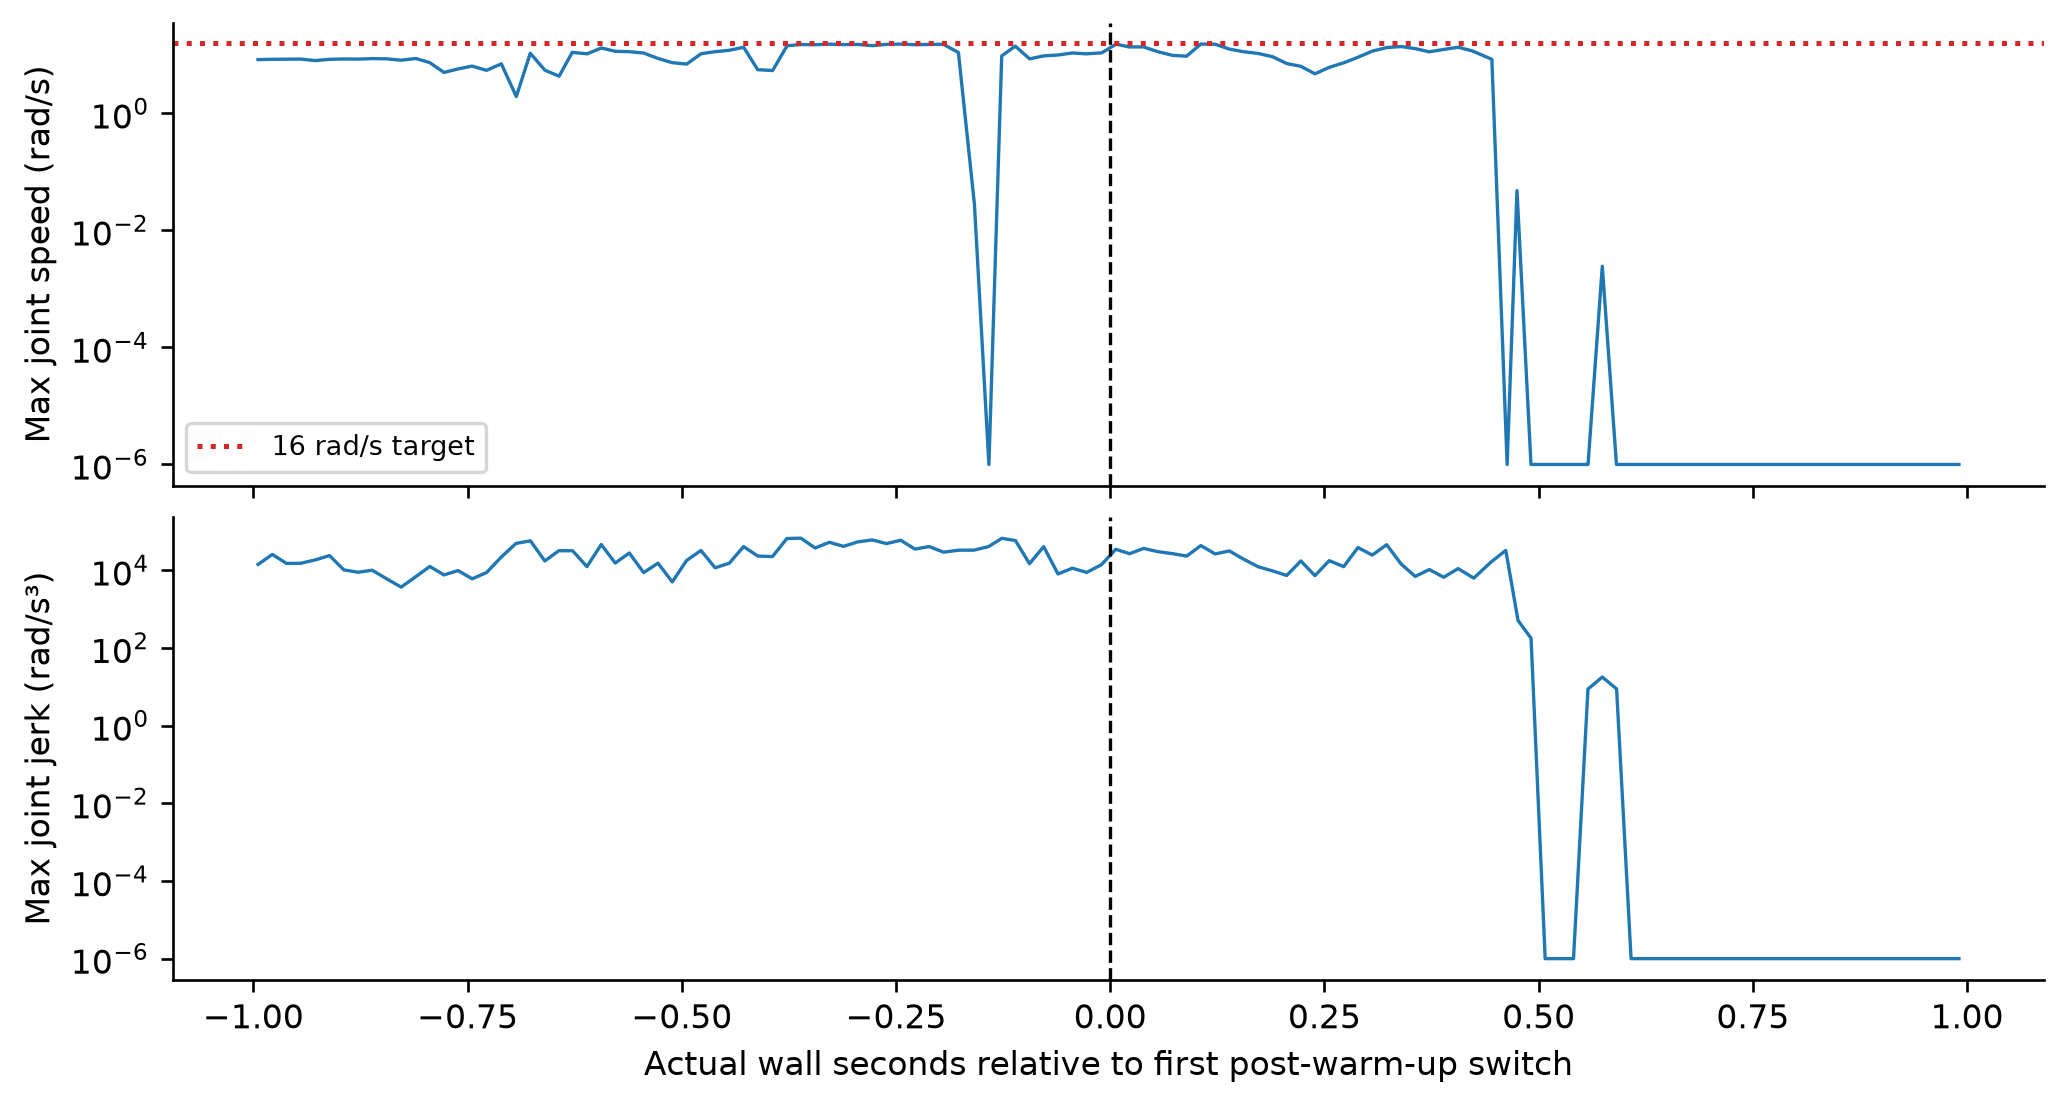
\includegraphics[width=\linewidth]{figures/chapter6_switch_dynamics.png}
\caption{Actual-clock speed and jerk around the first post-warm-up switch in
the fixed causal-full stitched seed-0 run. This is an illustrative trace, not an
average over independent transitions. Logarithmic axes retain large excursions.}
\label{fig:ch6_switch_dynamics}
\end{figure}

The corrected pipeline measures actual output intervals, constrains collision
projection by the remaining dynamic envelope and audits the emitted MuJoCo state.
The formal result supports RQ3 for the registered kinematic bounds at 60 Hz.
It remains a kinematic result: no torque, contact-force, balance or hardware
guarantee follows from these final-pose checks.

\section{Inference Time and End-to-End Response}

\subsection{Computation, preparation and control work}

\begin{table}[tb]
\centering\small
\input{experiment_results/reanalysis_rescue_60_v5/chapter6_tables/timing.tex}
\caption{Medians across runs of each run's query p95, control-work p99 and
deadline-miss ratio. Times are in ms. Failure counts apply the 16.67 ms p99 and
1\% deadline-miss targets to individual runs. These are not pooled frame
percentiles.}
\label{tab:ch6_timing}
\end{table}

\begin{figure}[tb]
\centering
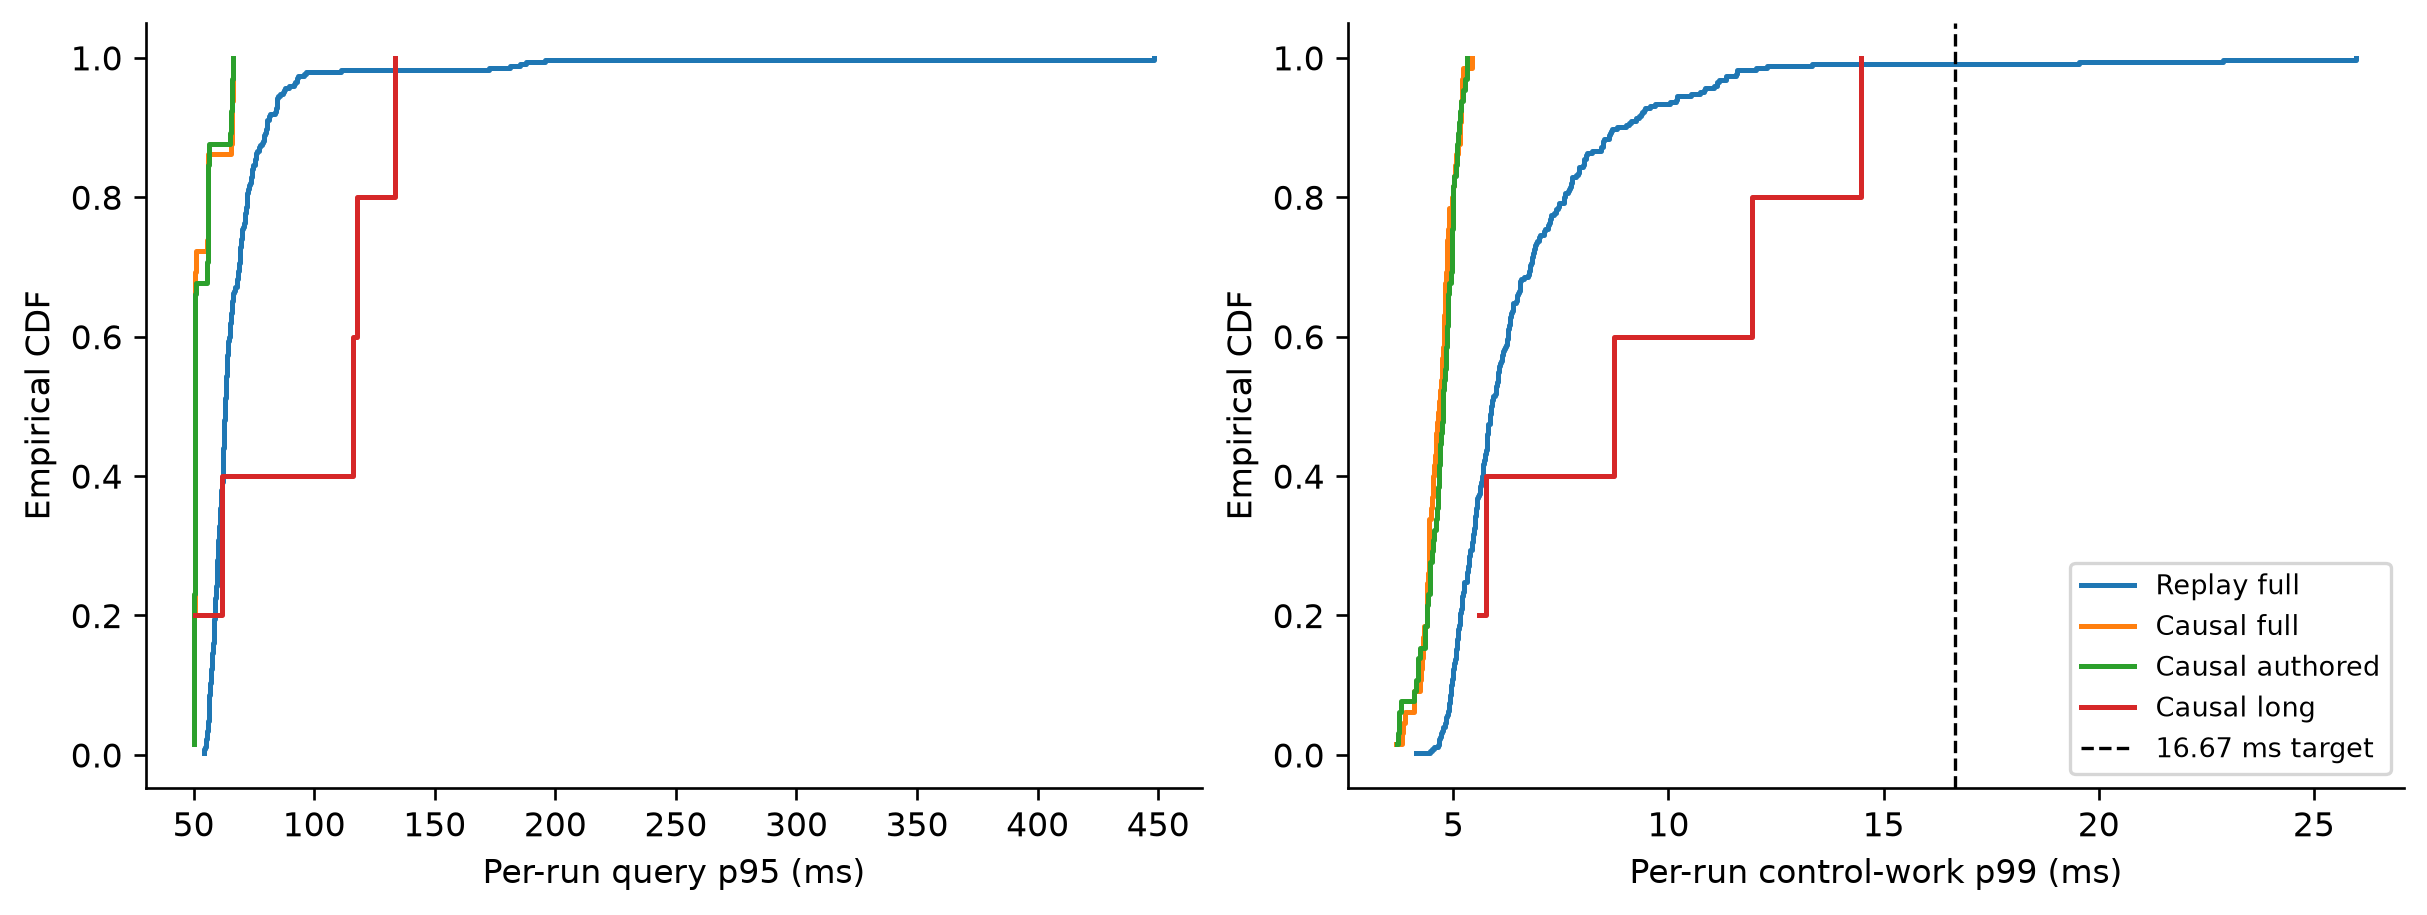
\includegraphics[width=\linewidth]{figures/chapter6_latency_cdf.png}
\caption{Empirical CDFs of per-run latency summaries, not individual query or
frame latencies. The right-hand reference line indicates the nominal 60 Hz
control period.}
\label{fig:ch6_latency}
\end{figure}

The causal short full-system median run-level query p95 is
\ChSixFullQuery{} ms, but its corresponding control-work p99 is
\ChSixFullWork{} ms (Table~\ref{tab:ch6_timing}). Retrieval latency and control
deadline compliance are therefore separate outcomes. The long-run median p99
is \ChSixLongWork{} ms and its median deadline-miss ratio is
\ChSixLongMiss{}. No formal 60 Hz run fails either real-time gate. The worst
individual long run remains below the registered limits, at 14.483 ms p99 and
0.00693 deadline-miss ratio. These are empirical Windows measurements rather
than a hard real-time scheduling guarantee.

\begin{table}[p]
\centering\small
\input{experiment_results/reanalysis_rescue_60_v5/chapter6_tables/stages.tex}
\caption{Stage-resolved timing for the causal full short suite. Each percentile
cell is the median across 65 runs of the within-run percentile, in ms. The last
column is the largest recorded maximum across runs. Nested
stages overlap, asynchronous stages execute concurrently with playback, and
percentiles cannot be added to obtain a total.}
\label{tab:ch6_stages}
\end{table}

\begin{table}[tb]
\centering\small
\input{experiment_results/reanalysis_rescue_60_v5/chapter6_tables/startup.tex}
\caption{Process-start measurements for the causal full short suite. These
startup durations are distinct from steady control work and are not controlled
OS-cache-cold measurements.}
\label{tab:ch6_startup}
\end{table}

Tables~\ref{tab:ch6_stages} and~\ref{tab:ch6_startup} distinguish ONNX execution,
hand-crafted features, track retrieval, motion ranking, candidate preparation
and control work. Candidate grounding and readiness are background operations.
Their wall-clock preparation latency is not an additional synchronous delay on
every control frame. However, asynchronous execution does not remove resource
contention or the need for a candidate to be ready when selected.

\begin{table}[tb]
\centering\small
\input{experiment_results/reanalysis_rescue_60_v5/chapter6_tables/readiness.tex}
\caption{Whole-run operational readiness counters. An underrun means the ready
pool is empty. A hold can occur even when other prepared motions exist. These
counters are not the post-warm-up frame totals used in the safety table.}
\label{tab:ch6_readiness}
\end{table}

The recorded ready-pool underrun and hold-last totals are both zero across all
135 causal formal runs (Table~\ref{tab:ch6_readiness}). The prepared-cache
fallback therefore meets the registered operational readiness targets in this
cohort, although it does not prove readiness for unseen catalogues or platforms.

The supplemental final-output audit performs an additional clearance check,
including forward kinematics. Its overhead is reported separately and remains
inside total control work. Thus differences from the old headless measurements
cannot be attributed solely to causal beat analysis. First-call/cold labels in
some stage counters also do not establish an OS-cache-cold benchmark. Complete
cold/warm distributions for every stage, and a separate mel-construction timer,
are not uniformly available. The chapter reports the timing actually recorded.

Submission attempts require particular care. While a retrieval worker is busy,
the control loop can attempt submission repeatedly before a successful update
advances the matching clock. Consequently, busy attempts divided by all attempts
are not automatically a one-second query-slot loss rate. A completed/submitted
ratio can also include one query still in flight at shutdown. The machine-readable
operational counters are retained, but a 99\% scheduled-slot completion claim is
not established from those counters alone.

\subsection{Musical changes and observable response}

\begin{figure}[tb]
\centering
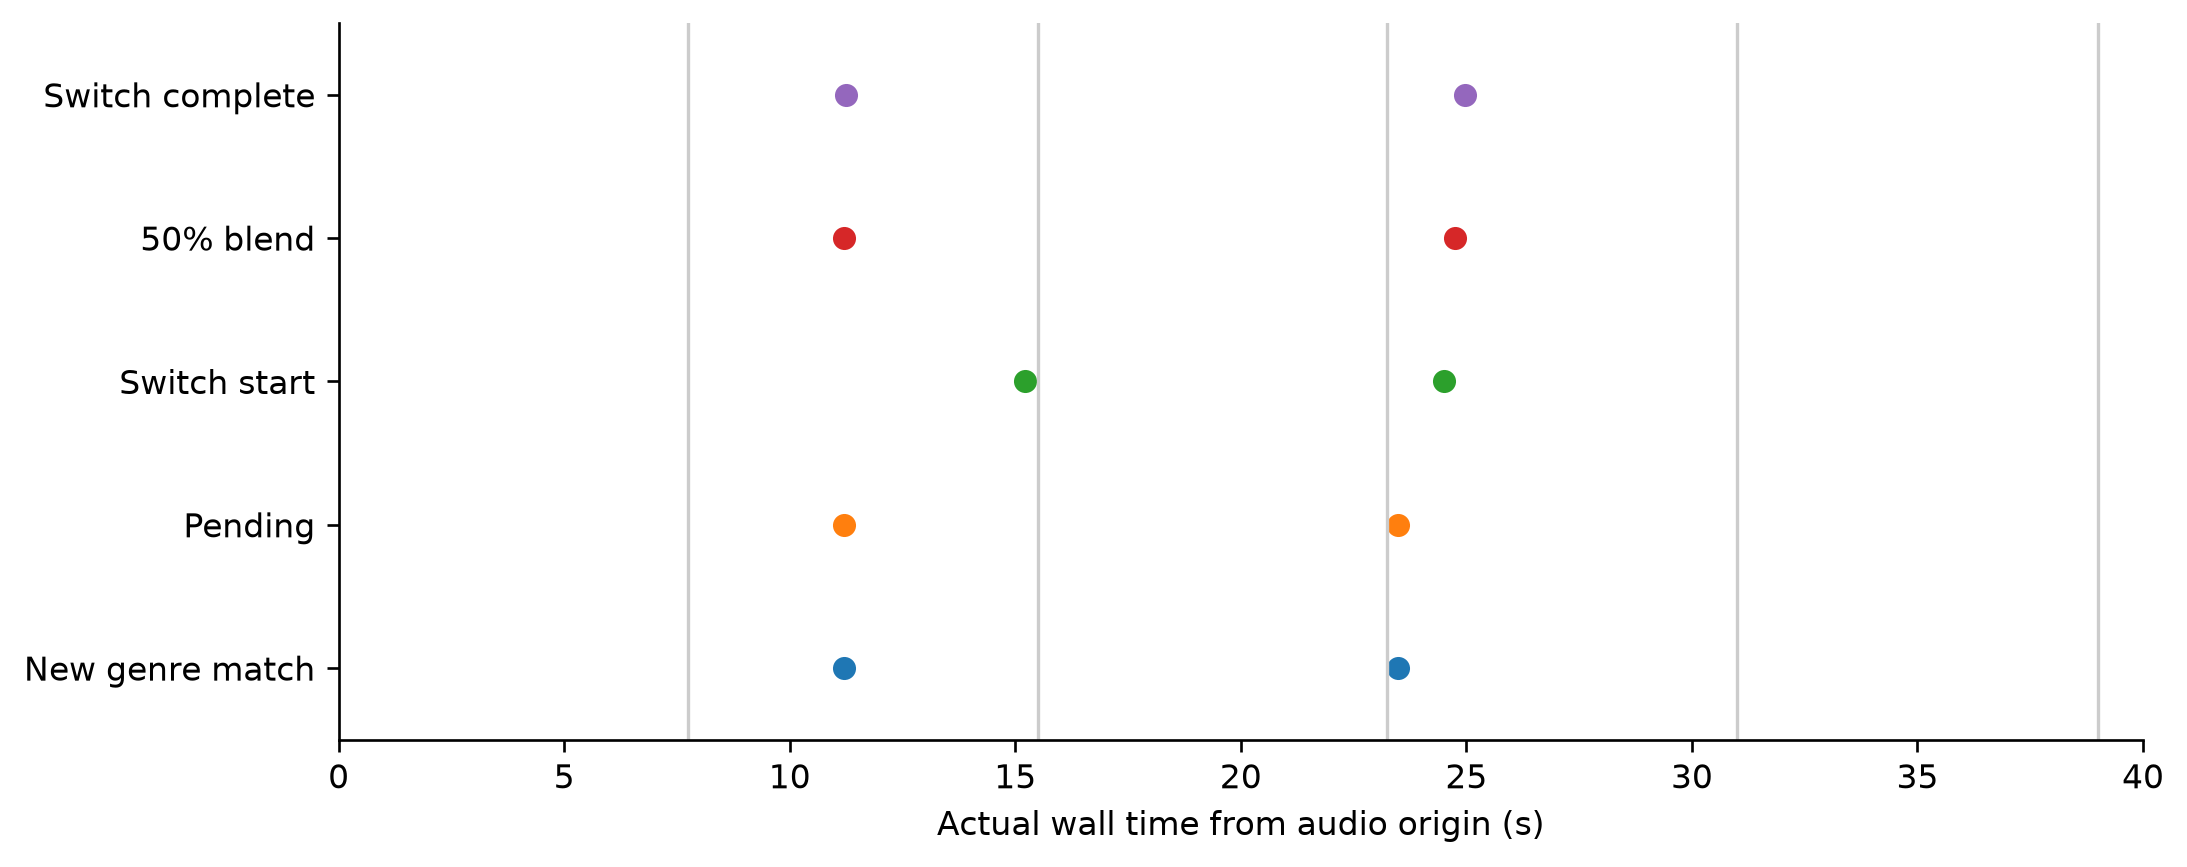
\includegraphics[width=\linewidth]{figures/chapter6_response_timeline.png}
\caption{Deterministically selected illustration: causal full, stitched source,
seed 0. Vertical lines mark source changes. Points mark observed milestones.
Responses are censored at the next change. An absent point is not a zero delay.}
\label{fig:ch6_response}
\end{figure}

Figure~\ref{fig:ch6_response} separates a new genre-compatible ranking from
pending selection, switch initiation, half blending and completion. Six seconds
of accumulated context are needed for the first query, and a post-change window
contains a mixture of old and new audio until that context has been replaced.
Query scheduling, repeated-winner evidence, bar boundaries and candidate readiness
can introduce further waiting. The six-second window is therefore neither an
ONNX inference time nor a universal fixed response latency.

Milestone traces are censored at the next musical change, including the repeated
stitched boundary in long runs. Genre-target matching is available for stitched
inputs. Tempo-jump and silence/recovery milestones are scheduling diagnostics,
not independently verified correct-tempo or correct-rejection responses. Pending
and switch events also need not refer to an identical candidate throughout a
complex change episode. These limitations prevent interpreting every observed
milestone chain as a successful semantic response. RQ4 is answered at the stage
and control-loop level, while fully attributed end-to-end responsiveness remains
a stricter future evaluation requirement.

\section{Ablation Study}

The replay ablations cover legacy retrieval, removal of motion compatibility,
instantaneous top-one selection, removal of bounded-hold diversity, authored
timing, fixed-entry/simple transitions, and disabling the output limiter. The
last condition is restricted to headless diagnostics. Collision checking remains
enabled. The causal supplement retests only the full/authored timing comparison,
not the complete eight-condition matrix.

\begin{table}[tb]
\centering\small
\input{experiment_results/reanalysis_rescue_60_v5/chapter6_tables/ablation.tex}
\caption{Selected paired ablation comparisons after source-level seed averaging.
$\Delta$ is ablation minus full. The Holm family includes all reported
condition-by-metric tests within the relevant suite, not only the selected rows
shown here. Replay jerk is a nominal-rate diagnostic.}
\label{tab:ch6_ablation}
\end{table}

Table~\ref{tab:ch6_ablation} evaluates the registered component hypotheses with
paired tests rather than treating 65 source/seed combinations as independent
music samples. A BAS benefit requires a direction favouring the full system and
support after multiplicity correction. A diversity benefit additionally needs
increased coverage or entropy without more than a 5\% mean relevance loss. A
beat-sync benefit must not increase deadline misses by more than one percentage
point. Absence of significance is not proof of equivalence, but it also does not
justify claiming a component effective because its mean moves in the expected
direction. RQ5 is therefore answered per component and per cohort, rather than by
declaring the entire architecture validated by the existence of an ablation.

In the selected replay comparisons, the apparent directions of retrieval recall,
selection entropy and nominal jerk do not survive Holm correction. In particular,
removing the diversity policy does not produce evidence of lower entropy under
this protocol. The causal authored comparison likewise supplies no corrected
evidence of a BAS difference. Its source-mean deadline-miss ratio differs from
full by \ChSixMissDifference{} (adjusted $p=\ChSixMissHolm{}$), and both
conditions pass the absolute 60 Hz gates. Thus the experiment establishes
neither a BAS benefit nor a deadline penalty for beat synchronisation.
Conditions were executed serially in a fixed matrix order, rather
than randomised across time. Background-load drift remains a possible timing
confound. Here ``causal'' describes audio availability, not a guarantee of
unconfounded causal inference about every performance difference.

\section{Long-Run Reliability}

All five causal long runs completed their registered duration, passed artifact
integrity and passed every evaluated real-time, readiness and final-output gate.
Repeating a 39-second source
for approximately ten minutes stresses recurrent switching and resource use,
but supplies only one source distribution.

The original long-run suite contains eight conditions, each at five seeds. Its
worst result must not be reported as if it belonged to the full system. Likewise,
the original full-system long runs cannot establish causal reliability because
their beat information and instrumentation differ from the supplement. The
causal long runs provide sustained evidence for the selected 60 Hz operating
point. They do not rescue the separate 120 Hz pilot, whose 15/21 failures show
that the original operating target is not reliable on this platform.

\section{Discussion by Research Question}

For RQ1, the leave-one-music-out shortlist provides stronger evidence than the
same-source motion sanity check, but top-one and rejection errors remain material.
For RQ2, rhythm alignment is measurable under a genuinely online delivery protocol,
yet it remains a proxy for musical timing and does not replace judged dance quality.
Coverage, entropy and reference-distribution diversity describe complementary
properties and should not be collapsed into an unrestricted diversity objective.

For RQ3, auditing final qpos verifies the registered end-to-end kinematic
constraints at 60 Hz while preserving the distinction from dynamics and hardware
safety. For RQ4, retrieval computation and asynchronous preparation are explicitly
measurable, and the selected 60 Hz operating point passes the empirical control
gates; the 120 Hz target does not. For RQ5, the paired
statistics delimit the component claims that can be made. Replay ablations and
causal timing ablations answer different experimental questions.

The appropriate overall conclusion is consequently conditional: Humanoid Matcher
is an auditable retrieval and playback pipeline that meets its registered
kinematic and empirical real-time contracts at 60 Hz on the measured platform.
It is not a hard-real-time or physically safe humanoid dance controller, and the
failed 120 Hz capacity test remains an engineering finding rather than evidence
to exclude.

\section{Limitations and Chapter Summary}

The evaluation has no human preference study, no dynamics-based tracking controller
and no hardware trial. BAS, FID/Div, foot-contact proxies and kinematic smoothness
cannot fully assess naturalness, expressiveness or dance aesthetics. The ten CC0
inputs and synthetic negatives provide limited external validity. Five seeds
increase repeatability evidence but do not multiply the number of independent
musical sources.

Further limitations arise from measurement granularity. The original actual
frame clocks cannot be recovered. Low-frequency traces approximate SMPL phase
and transition reconstruction, Cyclic ground truth differs from continuous human
choreography. And query-slot accounting is not identical to repeated submission
attempt accounting. These are stated explicitly rather than hidden behind a
single inference-time or quality number.

This chapter establishes a reproducible record of what the system retrieves,
how its outputs align with delivered beats, where its computation is spent, and
which operating point satisfies the output and timing constraints. Future work
should reduce collision-stage cost if 120 Hz remains a requirement, improve
scheduled-slot and candidate attribution, broaden rejection recordings, and
evaluate closed-loop tracking and human-perceived dance quality. Those extensions
require new evidence. They are not implied by the present kinematic experiments.
